L'implémentation de la vision artificielle change profondément les
pratiques des historien.nes en leur offrant de nouveaux outils pour
analyser rapidement et à grande échelle des corpus d'images. La machine
devient capable d'identifier des motifs spécifiques et de les relier à
d'autres sources, mettant à jour des réseaux et des narratifs complexes.

Le choix d'une architecture de réseau de neurones repose sur plusieurs
considérations~: la nature spécifique des données à traiter, la tâche
particulière à accomplir, et l'efficacité computationnelle visée. Le
défi consiste à trouver l'équilibre optimal entre l'efficacité de
l'implémentation et la performance sur les données visées, car chaque
type de réseau possède des caractéristiques et des avantages propres qui
le rendent plus ou moins adapté à des contextes particuliers.

Prenons pour exemple les trois tâches implémentées dans la plateforme
\eida et les questionnements qui ont motivé le choix d'une architecture.

\hypertarget{detection}{%
\subsection{YOLOv5 pour la détection~: performance et
légèreté}\label{detection}}

La tâche de détection d'objet consiste à identifier et localiser des
objets d'intérêt dans une image. Cette tâche comprend deux sous-tâches
principales~: déterminer la classe de chaque objet détecté (ici, le
diagramme) et localiser l'objet. Contrairement à la segmentation, la
détection ne classe pas les pixels individuellement mais identifie des
zones contenant chaque instance d'objet. En d'autres termes, elle ne
délimite pas précisément l'objet au niveau des pixels, mais dessine une
boîte (\emph{boulding-box}) autour de celui-ci.

Pour la reconnaissance et la classification d'objets dans des images,
les réseaux de neurones traditionnellement utilisés sont les \textsc{cnn}
(\emph{Convolutional Neural Network} ou réseau de neurone
convolutionnel). Ces architectures sont composés de deux types de
neurones agencés en plusieurs couches~: les neurones de traitement et
les neurones de mise en commun des sorties, dits de \textit{pooling}. Ils
procèdent de fait en plusieurs étapes~: l'extraction de \emph{features}
des données d'entrée (phase de traitement), l'agrégation de ces
\emph{features} (phase de pooling), puis la résolution du problème (dans
ce cas précis, la détection des objets).\footcite[p.680-681]{indolia_conceptual_2018}

          \begin{figure}[H]
          \begin{center}
          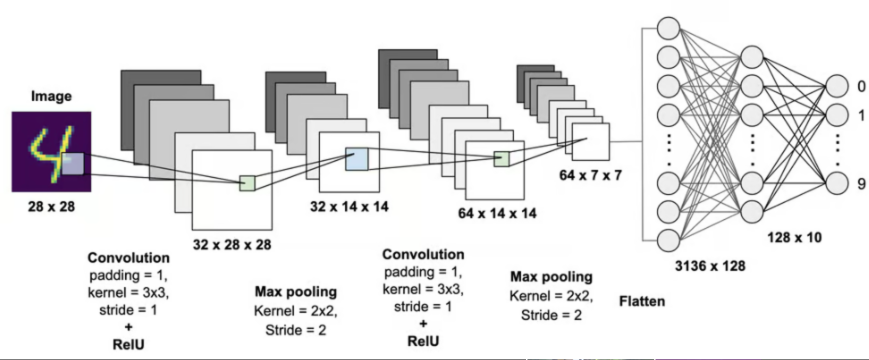
\includegraphics[height=7cm]{figues/CNN.png}
          \end{center}
          \caption{Fonctionnement d'un \cnn.\footcite{noauthor_intuitive_2016}}
          \label{fig:cnn} \end{figure}

Les neurones de traitement des \cnns sont organisés en couches
successives. Les premières couches apprennent à détecter des
caractéristiques simples (bords et textures par exemple), tandis que les
couches plus profondes combinent ces caractéristiques pour reconnaître
des formes plus complexes (visages et objets par exemple).

De plus, le \cnn utilise un filtre convolutif, soit une matrice de
valeurs qui sert à l'extraction des \emph{features}. Il faut imaginer ce
filtre comme une petite fenêtre qui glisse sur l'image. À chaque
position, il calcule une valeur en multipliant les valeurs des pixels
sous la fenêtre par les nombres correspondants du filtre et en
additionnant les résultats. Les filtres convolutifs sont appliqués à
toute l'image, ce qui permet de détecter une même caractéristique quelle
que soit sa position dans l'image. Cette propriété est appelée
\emph{invariance par translation}\footcite[p.48]{charniak_introduction_2021}.

Un filtre partage les mêmes poids sur toute l'image et pour une couche
donnée, de cette manière les \cnns réduisent considérablement le nombre de
paramètres à apprendre par rapport à un réseau de neurones entièrement
connecté. Cela les rend plus efficaces en termes de calcul et moins
sujets au sur-apprentissage.

Ces propriétés (hiérarchie d'extraction, invariance par translation et
partage des poids) améliorent la performance du réseau sur les
images.\footcite[p.680]{indolia_conceptual_2018}. C'est
à ce titre qu'un \cnn est employé pour la tâche de détection. \yolov,
publié en 2020, est la cinquième version du modèle de détection d'objet
et de segmentation d'images \yolo, développé à
l'Université de Washington Joseph Redmon et Ali Farhadi et lancé en
2015. \yolo se distingue par son unique étape de détection. Cette
subtilité change la donne, le rendant particulièrement rapide et
précis\footcite[p.7]{buttner_cordeep_2022}. Le modèle
fonctionne en temps réel et peut être utilisé sur \cpu classique.

\begin{kwote}                 
Current detection systems repurpose classifiers to perform detection. To
detect an object, these systems take a classifier for that object and
evaluate it at various locations and scales in a test image. Systems
like deformable parts models (DPM) use a sliding window approach where
the classifier is run at evenly spaced locations over the entire image.
More recent approaches like R-CNN use region proposal methods to first
generate potential bounding boxes in an image and then run a classifier
on these proposed boxes. After classification, post-processing is used
to refine the bounding boxes, eliminate duplicate detections, and
rescore the boxes based on other objects in the scene. These complex
pipelines are slow and hard to optimize because each individual
component must be trained separately. We reframe object detection as a
single regression problem, straight from image pixels to bounding box
coordinates and class probabilities. Using our system, you only look
once (\yolo) at an image to predict what objects are present and where
they are. \yolo is refreshingly simple~: {[}\ldots{]} A single
convolutional network simultaneously predicts multiple bounding boxes
and class probabilities for those boxes.\footcite[p.1]{redmon_you_2016}
                       \end{kwote}

En outre, son implémentation se veut aisée~: \yolov, contrairement à ses
prédécesseurs, est directement implémenté dans PyTorch\footnote{PyTorch est une
bibliothèque Python open-source. Permettant la représentation des
données sous forme de tenseurs (équivalents multidimensionnels des
matrices NumPy), elle permet l'entraînement des réseaux de neurones.},
permettant une intégration facile à un environnement de développement,
puisqu'il nécessite moins d'adaptation que les versions précédentes
fonctionnant avec le \textit{framework} Darknet, basé sur le langage
C\footcite[p.44]{norindr_traitement_2023}.

Pour conclure, \yolo est un choix qui allie performance et légèreté. Les
\cnns sont traditionnellement choisis pour les tâches de détections de
motifs dans des images, en raison de leur performance dans ce domaine.
En outre \yolo est un modèle dit \emph{off-the-shelf}~: généraliste,
réutilisable et simple d'implémentation, ce choix réduit les coûts de
conception, de fabrication et de maintenance.

L'extraction permet ainsi d'isoler les éléments graphiques pertinents
(diagrammes ou illustrations) au sein de grands corpus de documents.
Leur traitement automatisé en \textit{batch} offre une scalabilité élevée. En
outre, l'extraction des unités sémantiques de base offre une granularité
plus fine pour appliquer par la suite de nouveaux traitements (recherche
de similarité ou vectorisation).

\hypertarget{similarite}{%
\subsection{Similarité}\label{similarite}}

Le choix d'un réseau de neurones pour la recherche de similarité entre
les diagrammes extraits dépend de ce que l'on entend par similarité~:
elle peut être sémantique ou purement graphique, concerner un motif
particulier ou un style global\footcite[``Quelle similarité chercher~?
  De multiples échelles sont possibles~: celle du document
  (reproductions, duplicatas)~; celle de l'objet (reconnaissance d'un
  élément récurrent)~; celle du « style »~; ou même celle du motif
  (orientation d'un bras, position d'un corps, type de mise en
  page,\ldots)''][p.3]{champenois_visual_2023}, et peut
être mesurée de différentes manières\footcite{di_leonardo_visual_2016}.

L'évaluation des similarités visuelles au sein d'un très grand corpus
d'images implique en premier lieu une transformation des images en
représentations numériques appropriées. Une approche classique consiste à
transformer les images en représentations vectorielles basées sur les valeurs de pixels. Ces
vecteurs servent de base au calcul de métriques de
similarité.\footcite[Les explications qui suivent s'inspirent de la
  présentation donnée par Ségolène Albouy lors de la conférence \eida
  2024][]{noauthor_eida_nodate}.

Plusieurs approches permettent cette comparaison (par exemple le produit
scalaire ou la distance euclidienne)\footcite{gronne_introduction_2022}. Cependant,
la méthode la plus fréquemment utilisée en vision artificielle est la
\emph{cosine distance}. Cette approche consiste à calculer le cosinus de
l'angle entre les deux vecteurs à comparer. La méthode est
particulièrement efficace car elle évalue l'orientation des vecteurs
plutôt que leur magnitude, offrant ainsi une mesure de similarité
relative, plus robuste. Cette métrique est particulièrement adaptée aux
espaces vectoriels de haute dimension (plus de deux) et est largement
utilisée en vision par ordinateur.

Elle ne donne toutefois pas de résultats optimaux quand elle est
calculée sur une représentation basée sur les valeurs de pixels. Une
représentation intermédiaire d'une image via un modèle par extraction
des \emph{features} constitue une représentation plus optimale de
l'image. Les réseaux de neurones, conçus initialement pour des tâches de
classification ou de détection d'objets, peuvent être réutilisés pour
l'extraction de caractéristiques. En effet, les couches intermédiaires
contiennent des représentations de plus en plus abstraites de l'image.
Ces vecteurs de caractéristiques (ou \emph{feature vectors}), de
dimensionnalité réduite par rapport à la représentation pixellique,
condensent l'information visuelle pertinente pour comparaison.

Ce que capturent les \emph{features} au sein de l'image est assez
insaisissable, néanmoins l'utilisation de la \emph{cosine distance} sur
ces vecteurs permet de mesurer l'alignement sémantique entre deux
images, au-delà des simples similarités visuelles de bas
niveau\footcite{farley_multimodal_2024}.

En choisissant le bon extracteur pour les \emph{features} (la
\emph{backbone}\footnote{La \textit{backbone} est chargé d'extraire les \textit{features} de l'image. Elle sert de base sur laquelle sont construites les couches supérieures du réseau, qui sont souvent spécifiques à une tâche particulière (classification, détection d'objets, segmentation). Les backbones sont souvent pré-entraînés sur d'énormes ensembles de données, ce qui leur permet de capturer les caractéristiques générales sur le monde visuel. Elles peuvent ensuite être réutilisés comme point de départ pour de nombreuses autres tâches, accélérant ainsi le processus d'apprentissage et le développement d'architectures spécifiques.} ou \emph{feature net})\footnote{\eida
  utilise MoCo (\cite{he_momentum_2020}), une architecture
  convolutionnelle construite pour un apprentissage non-supervisé.} et la bonne couche\footnote{Dans le cas présent la
  quatrième couche convolutionnelle.}, la pertinence des vecteurs
descripteurs se trouve optimisée.

Cette approche, cependant, n'est toujours pas suffisante pour capturer
des éléments visuels répétés, indépendemment du style et de la forme
exacte. Pour pallier à cette limite, il est possible d'utiliser la méthode Segswap\footcite{shen_learning_2022}. Initialement
développée pour la recherche en histoire de l'art, cette méthode a été
éprouvée sur l'analyse des œuvres issues des ateliers de Brueghel~: ses
assistants étaient connus pour répéter des petits motifs d'un tableau à
l'autre. Le modèle prend deux images en entrée et renvoie un masque~: un
vecteur de correspondance qui \emph{map} les deux parties de l'image qui
se répètent.

Cependant, l'application de l'algorithme Segswap à l'ensemble des paires
d'images nécessite trop de ressources computationnelles. Pour optimiser
le processus, il a été mis en place une approche hybride. Dans un
premier temps, le score de \emph{cosine distance} entre les
\emph{feature vectors} est calculé pour toutes les paires d'images.
Cette étape permet de filtrer les paires d'images les moins susceptibles
de contenir des motifs récurrents, réduisant ainsi considérablement le
nombre de paires à soumettre à l'algorithme Segswap. Dans un second
temps, l'algorithme Segswap est appliqué uniquement aux paires d'images
ayant obtenu les scores de similarité cosinus les plus élevés.

Cette approche permet retrouver les variantes d'un même diagramme au fil
des copies et des éditions, alignant ainsi plusieurs témoins en vue
d'une édition critique. Les chercheur.ses pourront aussi s'appuyer sur
Segswap pour retrouver les variations d'un même élément graphique,
permettant de comparer les conventions visuelles en diachronie.
L'utilisation de la vision artificielle rend la tâche réalisable sur une
très grande base de donnée, ouvrant la voie à des études comparatives à
grande échelle.

Cependant, ces algorithmes ne ramèneront pas les similarités dites
``topologiques''\footnote{La transformation topologique d'un diagramme
  n'affecte pas son contenu mathématique. À une démonstration textuelle
  peuvent correspondre plusieurs représentations géométriques. Deux
  diagrammes peuvent donc être aspectuellement différent mais
  substanciellement équivalents.}. La vectorisation ouvre des
perspectives pour une analyse plus fine des composants des diagrammes,
afin de détecter les relations structurelles sous-jacentes.

\hypertarget{la-vectorisation-les-transformers}{%
\subsection{La vectorisation~: les
\emph{transformers}}\label{la-vectorisation-les-transformers}}

L'implémentation de la vectorisation permet d'extraire automatiquement
l'information géométrique contenue dans les diagrammes dans un format
léger et sémantiquement riche. Les représentations vectorielles sont en
effet significativement plus compactes que leurs homologues
matricielles. Elle sont stockées dans un fichier appelé \svg pour
\emph{Scalable Vector Graphic}. Ce format utilise le langage \xml pour
encoder la représentation vectorielle du diagramme. Les \svgs offrent en
outre une représentation du contenu de l'image indépendante de sa
résolution. Cette invariabilité est rendue possible par l'utilisation de
primitives géométriques (formes de base) et de leurs paramètres, plutôt
que de pixels, pour encoder l'image\footcite{noauthor_tutoriel_2024}. Dans
le cas présent, trois types de primitives sont utilisés~: les lignes,
cercles et arcs, qui constituent les formes fondamentales des
diagrammes du corpus \eida.

Chaque \emph{primitive} (forme géométrique élémentaire) est définie par
un ensemble de paramètres pour pouvoir être tracée. Un cercle est encodé
à l'aide de son rayon et des coordonnées de son centre~; la ligne est
définies par les coordonnées des points de départ et d'arrivée~; l'arc
par les coordonnées des points de départ, d'arrivée et du
\emph{midpoint}.

Cet encodage autorise un accès immédiat au contenu géométrique des
diagrammes, et permet une manipulation fine des éléments graphiques~: la
machine peut exploiter ce format en s'appuyant sur les valeurs
numériques qui définissent les primitives. L'implémentation de la
vectorisation dans la plateforme vise alors à fournir un outil efficace
pour étudier et analyser sémantiquement le contenu géométrique des
diagrammes, ouvrant la voie aux divers post-traitements sous-tendant
l'établissement d'une édition enrichie\footnote{Voir le \hypertarget{chapitre-6-vers-edition}{chapitre 6}}.

\emph{Quels défis présentent les sources~? Et quelles méthodes sont
adoptées en conséquence~?}

La conversion d'images \textit{raster} (matricielles, composées de pixels) de
dessins en images vectorielles est un problème déjà exploré dans le
domaine de la recherche en vision artificielle\footcite{egiazarian_deep_2020}. Les
premières approches séquentielles, impliquant un prétraitement en deux
étapes (filtrage, simplification et \emph{edge detection}\footcite{canny_computational_1986} suivi d'une
détection de primitives\footcite{ref-noauthor_ransac_nodate}, se sont
révélées efficaces sur des images de haute qualité. Cependant, ces
méthodes peinent à généraliser à des images plus complexes ou
bruitées\footcite{hilaire_robust_2006}.

Or le corpus d'\eida, composé de diagrammes astronomiques extraits de
manuscrits historiques, présente des défis spécifiques qui compliquent
leur traitement automatisé par les méthodes traditionnelles. Les
documents sont bien souvent détériorés (taches ou atténuation des
tracés)~; les traits manuels sont généralement irréguliers et présentent
des variations dans l'épaisseur et la clarté des lignes~; les diagrammes
peuvent être très simples comme présenter de nombreux traits
enchevêtrés. La principale difficulté réside dans la coexistence du
texte et des éléments graphiques. Le texte couvre fréquemment une partie
du contenu géométrique~; parfois même, les diagrammes sont superposés
avec des blocs de texte par manque de place\footcite{kalleli_historical_2024}.

La complexité de la donnée historique rend la tâche presque impossible
aux méthodes de traitement séquentielles trop fortement dépendantes d'une
détection des contours (première étape~: \emph{edge détection})
qualitative. Or les structures les plus fines sont souvent perdues lors
de cette étape, ou bien les résultats souffrent de bruit excessif. La
séquentialité accroît ainsi le risque d'erreurs cumulatives. D'autre
part, lors de la dernière étape, les motifs les plus petits\footnote{Il
  y a moins de pixels et \ransac se base sur le nombre de pixel pour la
  détection des formes.} ont de grandes chances d'être manqués. Il n'est
pas non plus possible d'appliquer un filtre sémantique aux détections,
et les bordures des document sont souvent détectées comme des lignes. La
dernière étape ralentit aussi considérablement le processus\footnote{la
  dernière étape de détection (cf.
  (\cite{noauthor_ransac_nodate}), détecte les
  primitives une par une.}. En outre, la méthode séquentielle requiert
une intervention humaine importante pour ajuster les paramètres en
fonction des caractéristiques spécifiques de chaque jeu de données.
Cette dépendance à l'expertise de l'utilisateur.rice restreint sa capacité de
généralisation et rend difficile son application à des corpus de
diagrammes hétérogènes.

Syrine Kalleli, doctorante à l'École des Ponts, propose une solution
basée sur un modèle de type \emph{transformers} pour remédier aux
problèmes posés par les méthodes classiques\footcite{kalleli_historical_2024}.

Les transformers se basent sur une une méthode d'apprentissage de type
\textit{Seq2Seq} et sur une bipartition structurelle (encodeur-décodeur).
L'apprentissage séquence à séquence est une technique
d'apprentissage profond permettant d'associer une séquence de symboles à
une autre séquence de symboles sans que cette mise en correspondance
soit basée sur les symboles en eux-mêmes. Son application par excellence
est la traduction automatique, mais elle connaît ces dernières années,
de plus en plus d'application dans le traitement de l'image\footcite{dosovitskiy_image_2021}. Elle
consiste à donner à la machine un corpus aligné, à savoir de
nombreux exemples de paires, et d'entraîner un modèle à retrouver
l'association. Le modèle opère en deux passes. La première, dont le but
est d'extraires les \emph{features} de l'image d'entrée, est appelée
passe d'encodage. La passe de décodage vise l'élément cible~: partant de
ces \emph{features}, elle prédit les primitives d'intérêt\footcite[p.90]{charniak_introduction_2021}.

          \begin{figure}[H]
          \begin{center}
          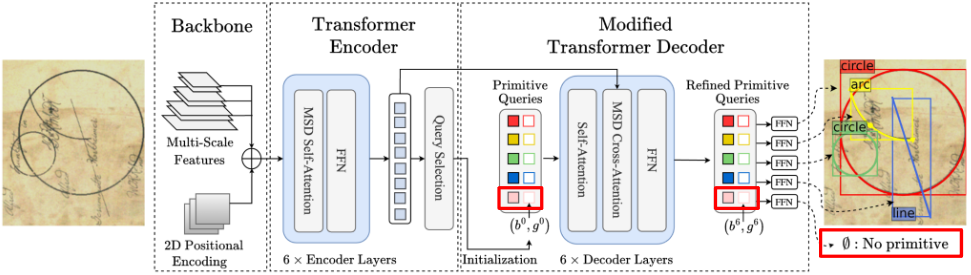
\includegraphics[height=4.5cm]{figues/transformers.png}
          \end{center}
          \caption{Fonctionnement de la méthode de vectorisation, basée sur les transformers.\footcite{kalleli_historical_2024}}
          \label{fig:vectorisation} \end{figure}

En outre, contrairement aux \cnns dont les performances reposent sur une
convolution séquentielle de l'image, les modèles \textit{seq2seq} doivent leur
efficacité à la notion d'\emph{attention}. Le mécanisme d'attention
confère au modèle la capacité de hiérarchiser l'information contenue
dans une image. En attribuant des poids variables aux différentes
régions de l'image, le modèle est en mesure de focaliser son traitement
sur les zones les plus pertinentes pour la tâche à accomplir, en
utilisant un ensemble de \emph{requêtes} (ou \emph{queries})\footcite[p.95]{charniak_introduction_2021}. Chaque requête correspond à une primitive parmi le triplet
initialement défini~: segment, arc et cercle\footcite{noauthor_eida_nodate}.

En somme, la méthode consiste à encoder l'image en représentations
sémantiques ou \emph{features}, et à effectuer un décodage des
\emph{features} en concentrant l'attention du modèle sur un ensemble de
motifs à détecter, en l'occurence trois types de primitives. Le modèle
ramène alors les coordonnées de ces primitives~: dans un premier temps,
elles sont stockées dans un format Numpy~: une structure de données
permettant la manipulation d'arrays multidimensionnels (Fig. \ref{fig:npz}). Post-inférence,
un script est capable de reconstituer les fichiers \svg au format \xml.

\begin{figure}
\begin{center}
\begin{verbatim}
    lines
[[134.81066895 457.17818451 779.38134766 248.8579483 ]
 [450.41806698 701.88641357 445.5779047   29.55957031]
 [ 82.28451538 235.88547516 751.17868042 460.67421722]
 [846.97953796 687.73287964 839.02302551  46.39743042]]
line_scores
[0.9833361  0.97366863 0.91139853 0.6446364 ]
circles
[[444.50769043 358.36816406 325.14129639]
 [122.31943512 357.18722534  99.33002472]
 [771.32922363 357.23934937 100.2789917 ]]
circle_scores
[0.9783766 0.955871  0.8885103]
arcs
[[720.67673302 494.20816517 745.99196815 474.5509901  740.33850098
  491.46079016]]
arc_scores
[0.31675324]
\end{verbatim}
\end{center}
\caption{Exemple de contenu d'un fichier \textsc{npz}}
          \label{fig:npz}
          \end{figure}


\begin{lstlisting}[language=xml, frame=single, breaklines=true, caption={exemple de contenu d'un fichier \svg}]
<?xml version='1.0' encoding='us-ascii'?>
<svg xmlns="http://www.w3.org/2000/svg" xmlns:xlink="http://www.w3.org/1999/xlink" baseProfile="tiny" height="2597" version="1.2" width="2460" xmlns:inkscape="http://www.inkscape.org/namespaces/inkscape" xmlns:sodipodi="http://sodipodi.sourceforge.net/DTD/sodipodi-0.dtd" inkscape:version="1.3 (0e150ed, 2023-07-21)">
  <defs />
  <image height="2597" width="2460" x="0" xlink:href="ms154_0139_1798,1606,2460,2597.jpg" y="0" />
  <circle cx="1265.9037" cy="1293.51" fill="none" r="506.6848" stroke="orange" stroke-width="3" />
  <circle cx="1260.7471" cy="1288.5127" fill="none" r="774.76514" stroke="orange" stroke-width="3" />
  <circle cx="1248.9653" cy="1293.2999" fill="none" r="1173.3875" stroke="orange" stroke-width="3" />
  <path d="M 947.62726 562.3929 L 2092.92 1338.452" fill="none" stroke="green" stroke-width="3" />
  <path d="M 91.71399 1291.111 L 2418.0642 1297.6548" fill="none" stroke="green" stroke-width="3" />
  <path d="M 1261.4149 2524.8396 L 1283.8896 109.190315" fill="none" stroke="green" stroke-width="3" />
  <path d="M 1819.7242 950.7695 L 1928.3906 1129.3221" fill="none" stroke="green" stroke-width="3" />
  <path d="M 1279.6703 109.75813 L 1633.5283 665.58594" fill="none" stroke="green" stroke-width="3" />
  <path d="M 792.355 186.13255 L 2428.4106 1307.5989" fill="none" stroke="green" stroke-width="3" />
</svg>
\end{lstlisting}


        
          \begin{figure}[H]
          \begin{center}
          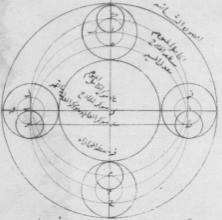
\includegraphics[height=4cm]{figues/vecto_init.png}
          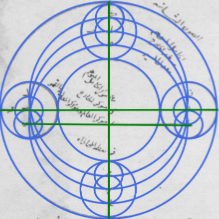
\includegraphics[height=4cm]{figues/vecto_results.png}
          \end{center}
          \caption{Résultat de la vectorisation.}
          \label{fig:results} \end{figure}

        


    